%%%%%%%%%%%%%%%%%%%%%%%%%%%%%%%%%%%%%%%%%
% Journal Article
% LaTeX Template
% Version 1.3 (9/9/13)
%
% This template has been downloaded from:
% http://www.LaTeXTemplates.com
%
% Original author:
% Frits Wenneker (http://www.howtotex.com)
%
% License:
% CC BY-NC-SA 3.0 (http://creativecommons.org/licenses/by-nc-sa/3.0/)
%
%%%%%%%%%%%%%%%%%%%%%%%%%%%%%%%%%%%%%%%%%

%----------------------------------------------------------------------------------------
%	PACKAGES AND OTHER DOCUMENT CONFIGURATIONS
%----------------------------------------------------------------------------------------

\documentclass[twoside]{article}

\usepackage{lipsum} % Package to generate dummy text throughout this template
\usepackage[sc]{mathpazo} % Use the Palatino font
\usepackage[T1]{fontenc} % Use 8-bit encoding that has 256 glyphs
\linespread{1.05} % Line spacing - Palatino needs more space between lines
\usepackage{microtype} % Slightly tweak font spacing for aesthetics

\usepackage[hmarginratio=1:1,top=32mm,columnsep=20pt]{geometry} % Document margins
\usepackage{multicol} % Used for the two-column layout of the document
\usepackage[hang, small,labelfont=bf,up,textfont=it,up]{caption} % Custom captions under/above floats in tables or figures
\usepackage{booktabs} % Horizontal rules in tables
\usepackage{float} % Required for tables and figures in the multi-column environment - they need to be placed in specific locations with the [H] (e.g. \begin{table}[H])
\usepackage{hyperref} % For hyperlinks in the PDF

\usepackage{graphicx}

\usepackage{lettrine} % The lettrine is the first enlarged letter at the beginning of the text
\usepackage{paralist} % Used for the compactitem environment which makes bullet points with less space between them

\usepackage{abstract} % Allows abstract customization
\renewcommand{\abstractnamefont}{\normalfont\bfseries} % Set the "Abstract" text to bold
\renewcommand{\abstracttextfont}{\normalfont\small\itshape} % Set the abstract itself to small italic text

\usepackage{titlesec} % Allows customization of titles
\renewcommand\thesection{\Roman{section}} % Roman numerals for the sections
\renewcommand\thesubsection{\Roman{subsection}} % Roman numerals for subsections
\titleformat{\section}[block]{\large\scshape\centering}{\thesection.}{1em}{} % Change the look of the section titles
\titleformat{\subsection}[block]{\large}{\thesubsection.}{1em}{} % Change the look of the section titles

\usepackage{fancyhdr} % Headers and footers
\pagestyle{fancy} % All pages have headers and footers
\fancyhead{} % Blank out the default header
\fancyfoot{} % Blank out the default footer
\fancyhead[C]{Vaccinating Health Professionals Before Patients $\bullet$ April 2021 $\bullet$ Vol. I, No. 1} % Custom header text
\fancyfoot[RO,LE]{\thepage} % Custom footer text

%----------------------------------------------------------------------------------------
%	TITLE SECTION
%----------------------------------------------------------------------------------------

\title{\vspace{-15mm}\fontsize{24pt}{10pt}\selectfont\textbf{The Effect of COVID-19 Vaccinating Health Professionals Prior to Patients }} % Article title

\author{
\large
\textsc{Jacob H, Lauren H, Ethan R, David W}\thanks{A thank you or further information}\\[2mm] % Your name
%\normalsize University of California \\ % Your institution
%\normalsize \href{mailto:john@smith.com}{john@smith.com} % Your email address
\vspace{-5mm}
}
\date{}

%----------------------------------------------------------------------------------------

\begin{document}

\maketitle % Insert title

\thispagestyle{fancy} % All pages have headers and footers

%----------------------------------------------------------------------------------------
%	ABSTRACT
%----------------------------------------------------------------------------------------

\begin{abstract}

\noindent \lipsum[1] % Dummy abstract text

\end{abstract}

%----------------------------------------------------------------------------------------
%	ARTICLE CONTENTS
%----------------------------------------------------------------------------------------

\begin{multicols}{2} % Two-column layout throughout the main article text

\section{Introduction}

\lettrine[nindent=0em,lines=3]{L} orem ipsum dolor sit amet, consectetur adipiscing elit.
\lipsum[2-3] % Dummy text

%------------------------------------------------

\section{Methods}

Maecenas sed ultricies felis. Sed imperdiet dictum arcu a egestas. 
\begin{compactitem}
\item Donec dolor arcu, rutrum id molestie in, viverra sed diam
\item Curabitur feugiat
\item turpis sed auctor facilisis
\item arcu eros accumsan lorem, at posuere mi diam sit amet tortor
\item Fusce fermentum, mi sit amet euismod rutrum
\item sem lorem molestie diam, iaculis aliquet sapien tortor non nisi
\item Pellentesque bibendum pretium aliquet
\end{compactitem}
\lipsum[4] % Dummy text

%------------------------------------------------

\section{Results}
\subsection{Mathematical Model}
\rule{\linewidth}{0.5pt}\\

\subsection{Nursing Home Trends over Time: Nationwide}

\begin{figure}[H]
	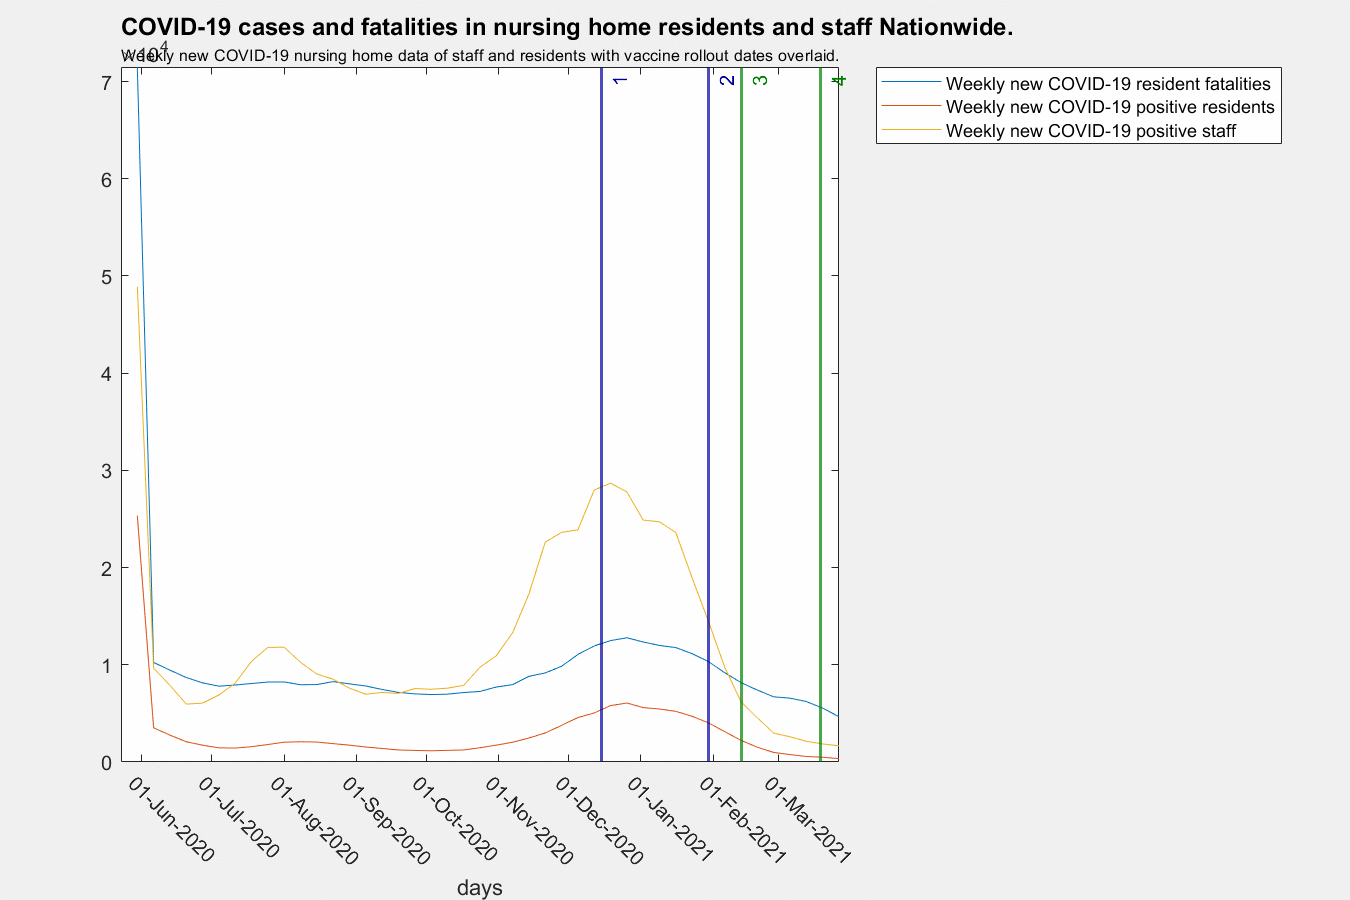
\includegraphics[width=\linewidth]{images/nationwide_nursing_home_with_vaccine.png}
	\caption{}
	\label{fig:images/nationwide_nursing_home_with_vaccineLabel}
\end{figure}
\rule{\linewidth}{0.5pt}\\
\subsection{Nursing Home Trends over Time: Statewide}

\begin{figure}[H]
	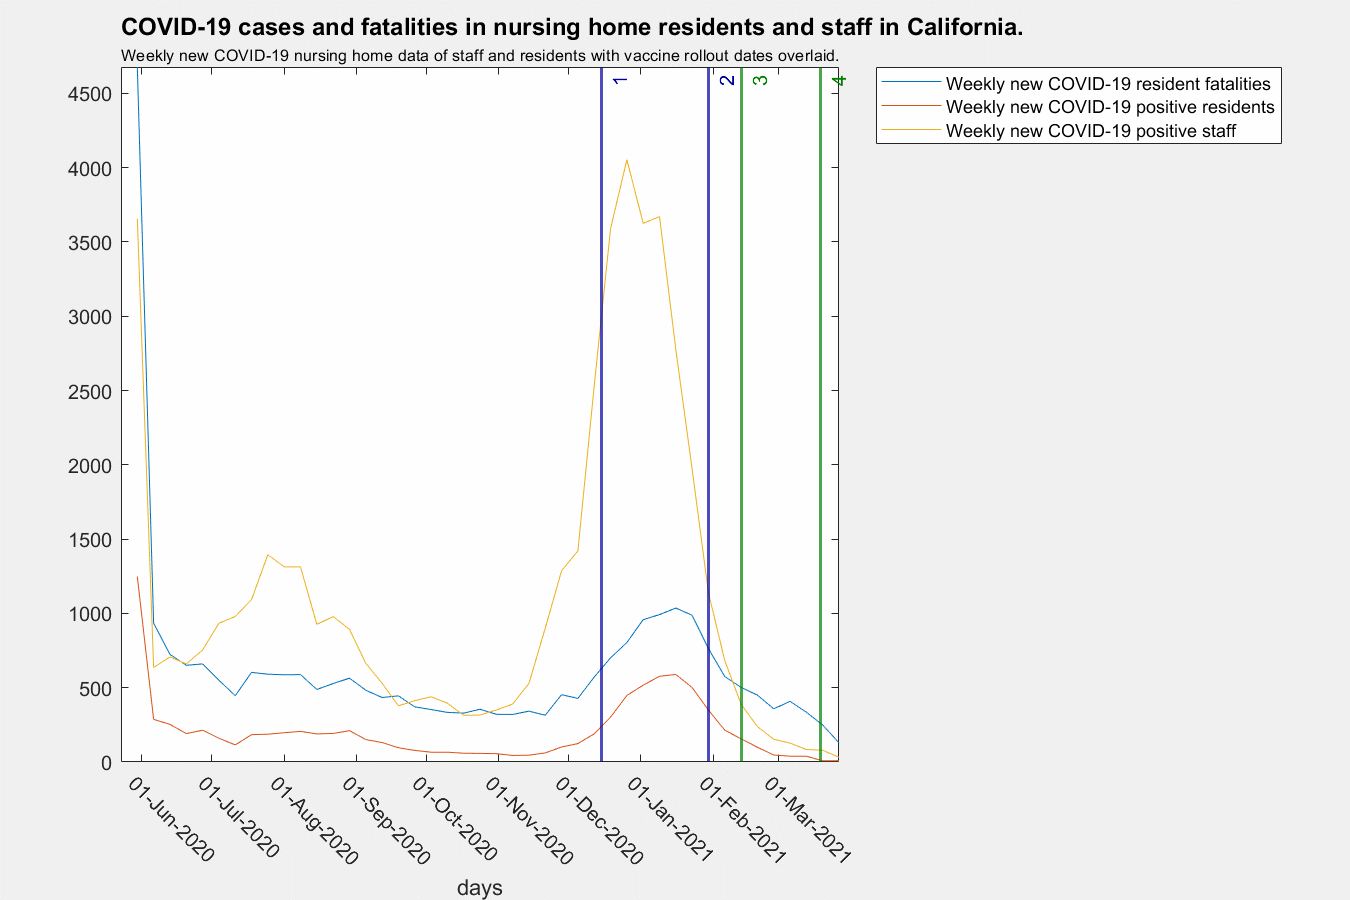
\includegraphics[width=\linewidth]{images/california_nursing_home_with_vaccine.png}
	\caption{}
	\label{fig:images/california_nursing_home_with_vaccineLabel}
\end{figure}

\begin{figure}[H]
	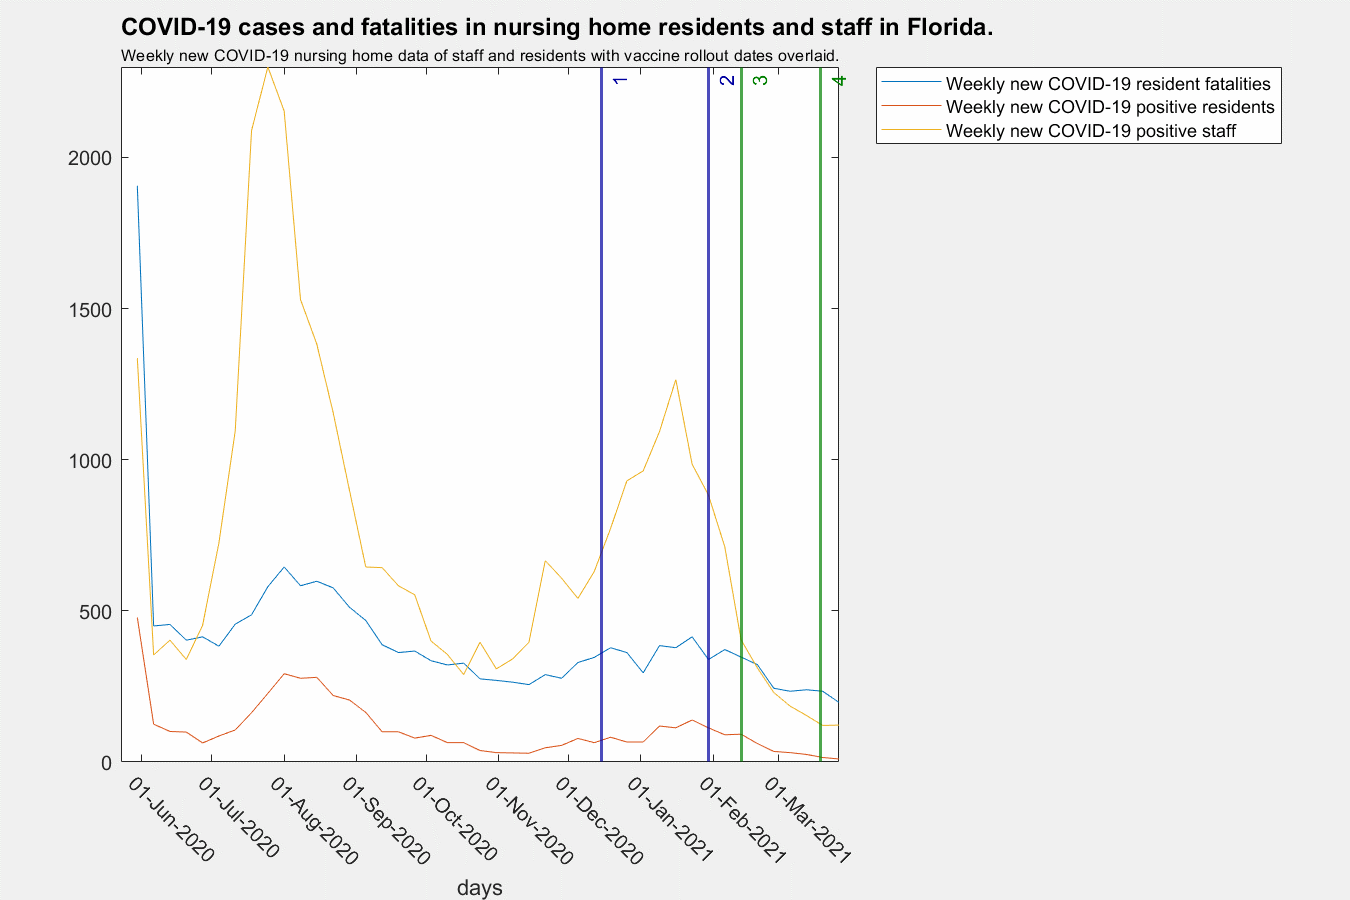
\includegraphics[width=\linewidth]{images/florida_nursing_home_with_vaccine.png}
	\caption{}
	\label{fig:images/florida_nursing_home_with_vaccineLabel}
\end{figure}

\begin{figure}[H]
	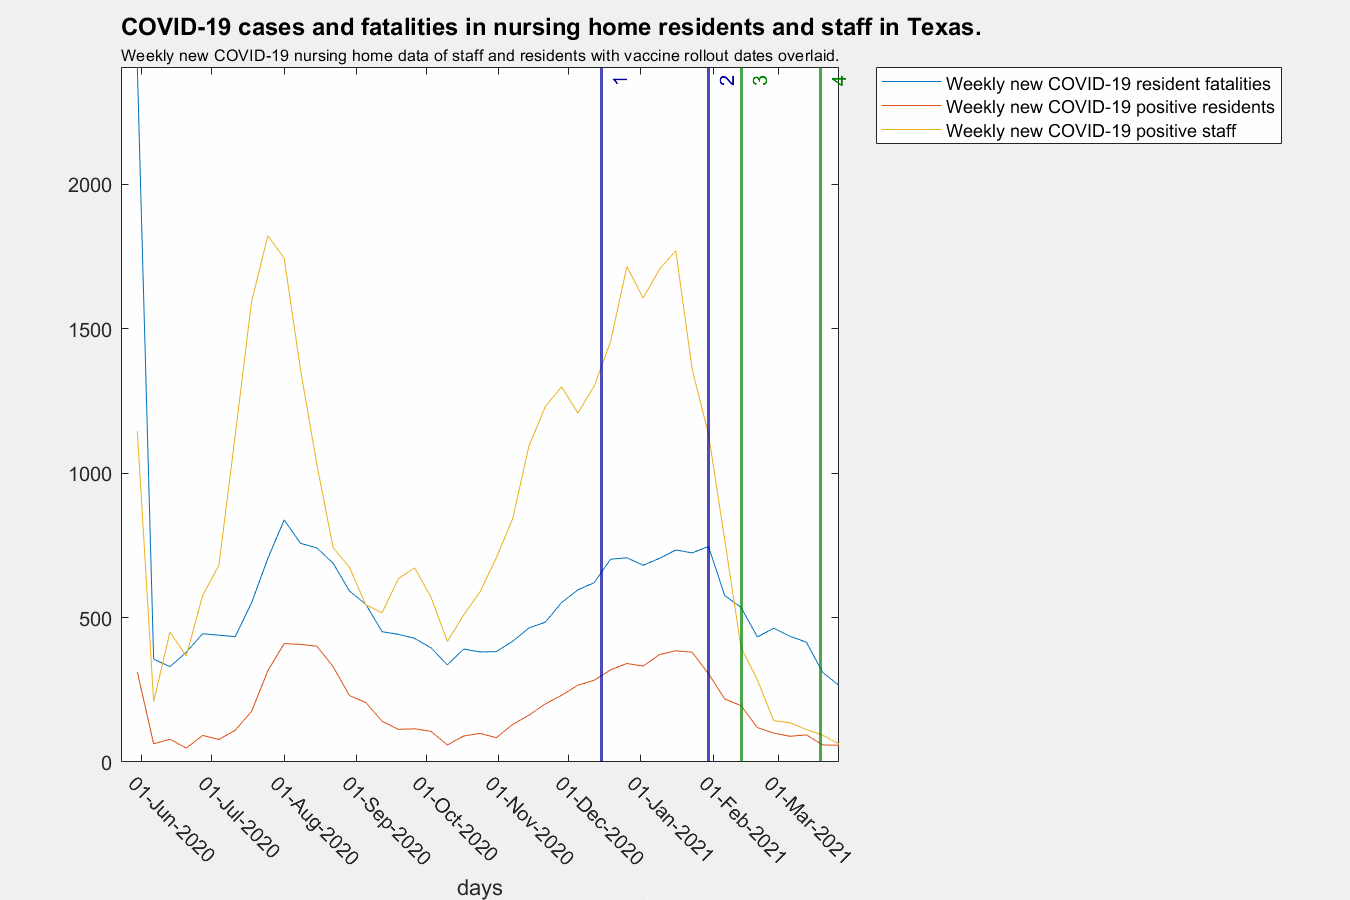
\includegraphics[width=\linewidth]{images/texas_nursing_home_with_vaccine.png}
	\caption{}
	\label{fig:images/texas_nursing_home_with_vaccineLabel}
\end{figure}
\rule{\linewidth}{0.5pt}\\
\subsection{Nursing Home Trends over Time: Countywide}

\begin{figure}[H]
	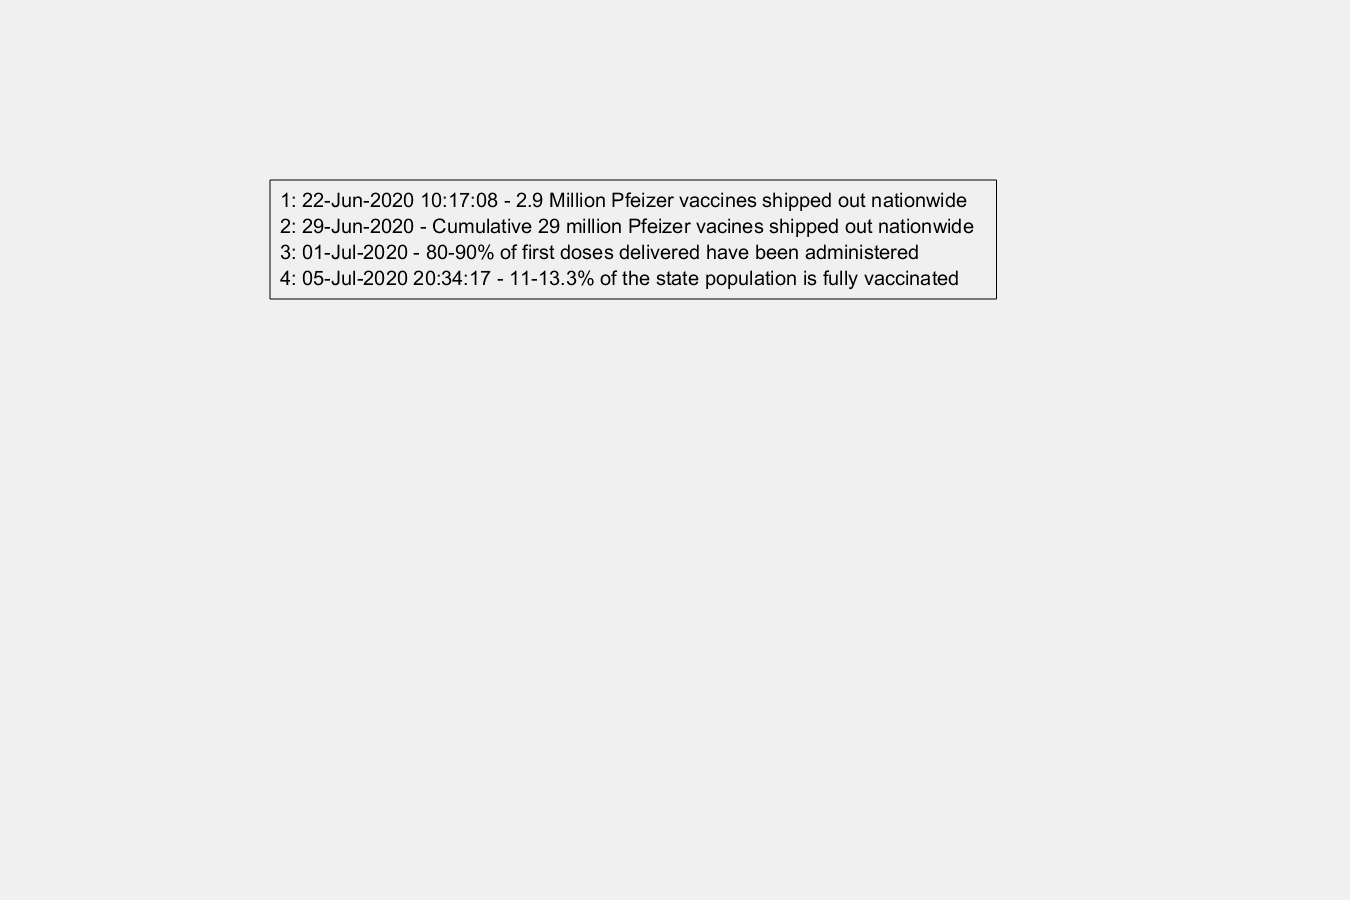
\includegraphics[width=\linewidth]{legends/new_vaccine_rollout_legend.png}
	\caption{}
	\label{fig:legends/new_vaccine_rollout_legendLabel}
\end{figure}


\begin{figure}[H]
	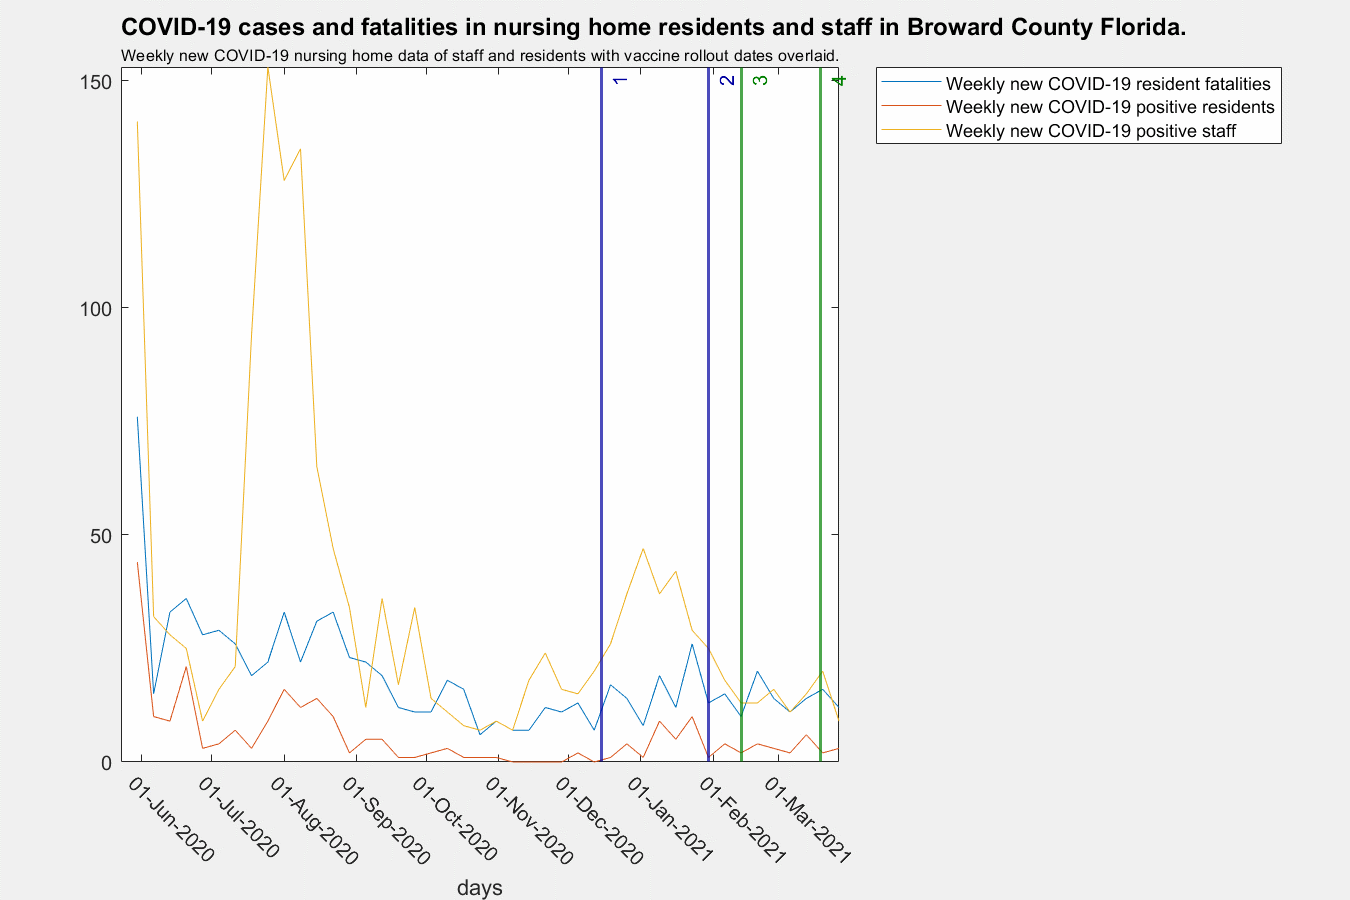
\includegraphics[width=\linewidth]{images/broward_nursing_home_with_vaccine.png}
	\caption{}
	\label{fig:images/broward_nursing_home_with_vaccineLabel}
\end{figure}

\begin{figure}[H]
	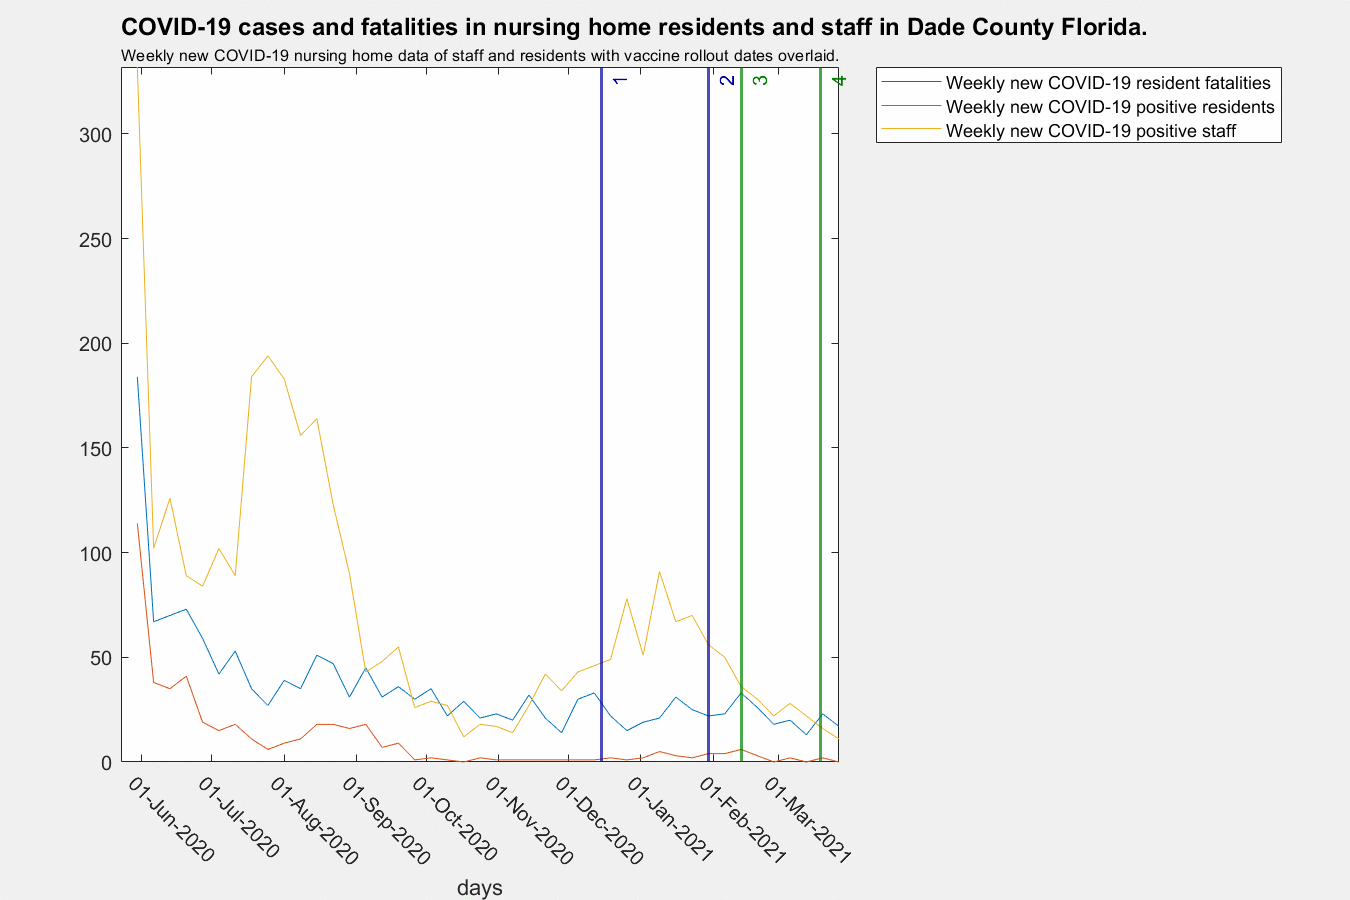
\includegraphics[width=\linewidth]{images/dade_nursing_home_with_vaccine.png}
	\caption{}
	\label{fig:images/dade_nursing_home_with_vaccineLabel}
\end{figure}

\begin{figure}[H]
	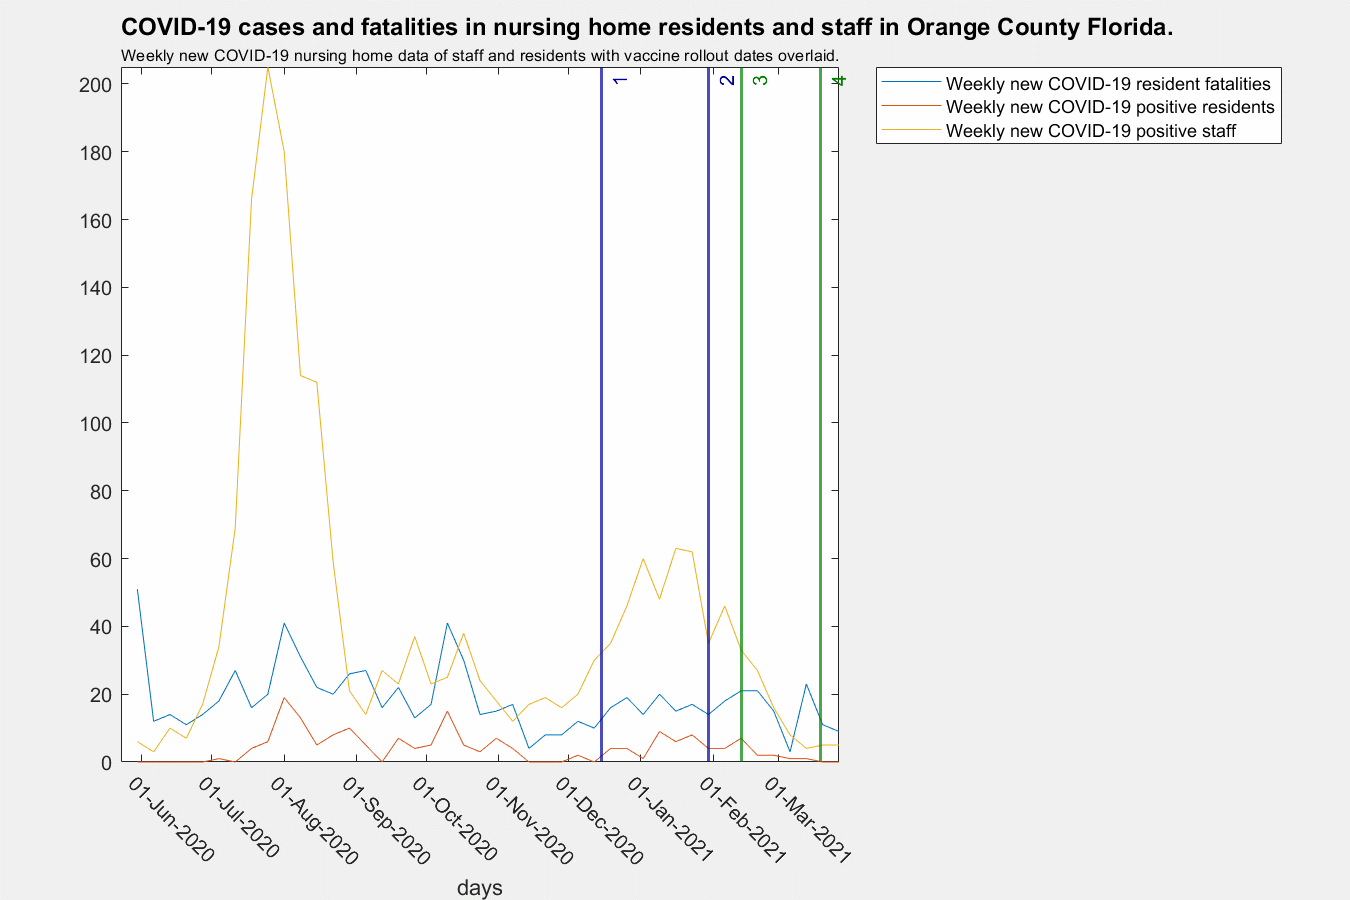
\includegraphics[width=\linewidth]{images/orange_nursing_home_with_vaccine.png}
	\caption{}
	\label{fig:images/orange_nursing_home_with_vaccineLabel}
\end{figure}

\begin{figure}[H]
	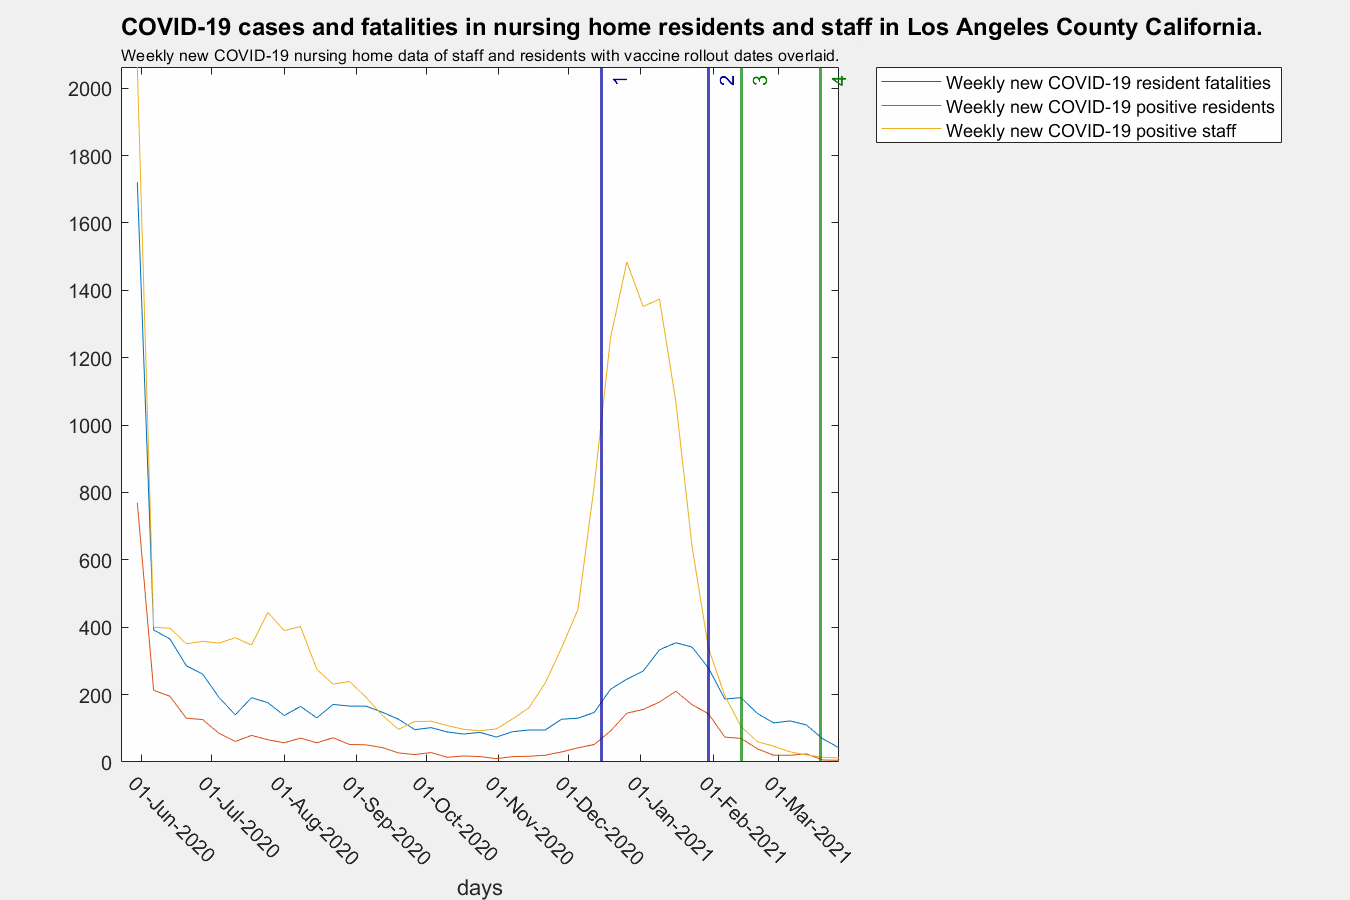
\includegraphics[width=\linewidth]{images/losangeles_nursing_home_with_vaccine.png}
	\caption{}
	\label{fig:images/losangeles_nursing_home_with_vaccineLabel}
\end{figure}

\begin{figure}[H]
	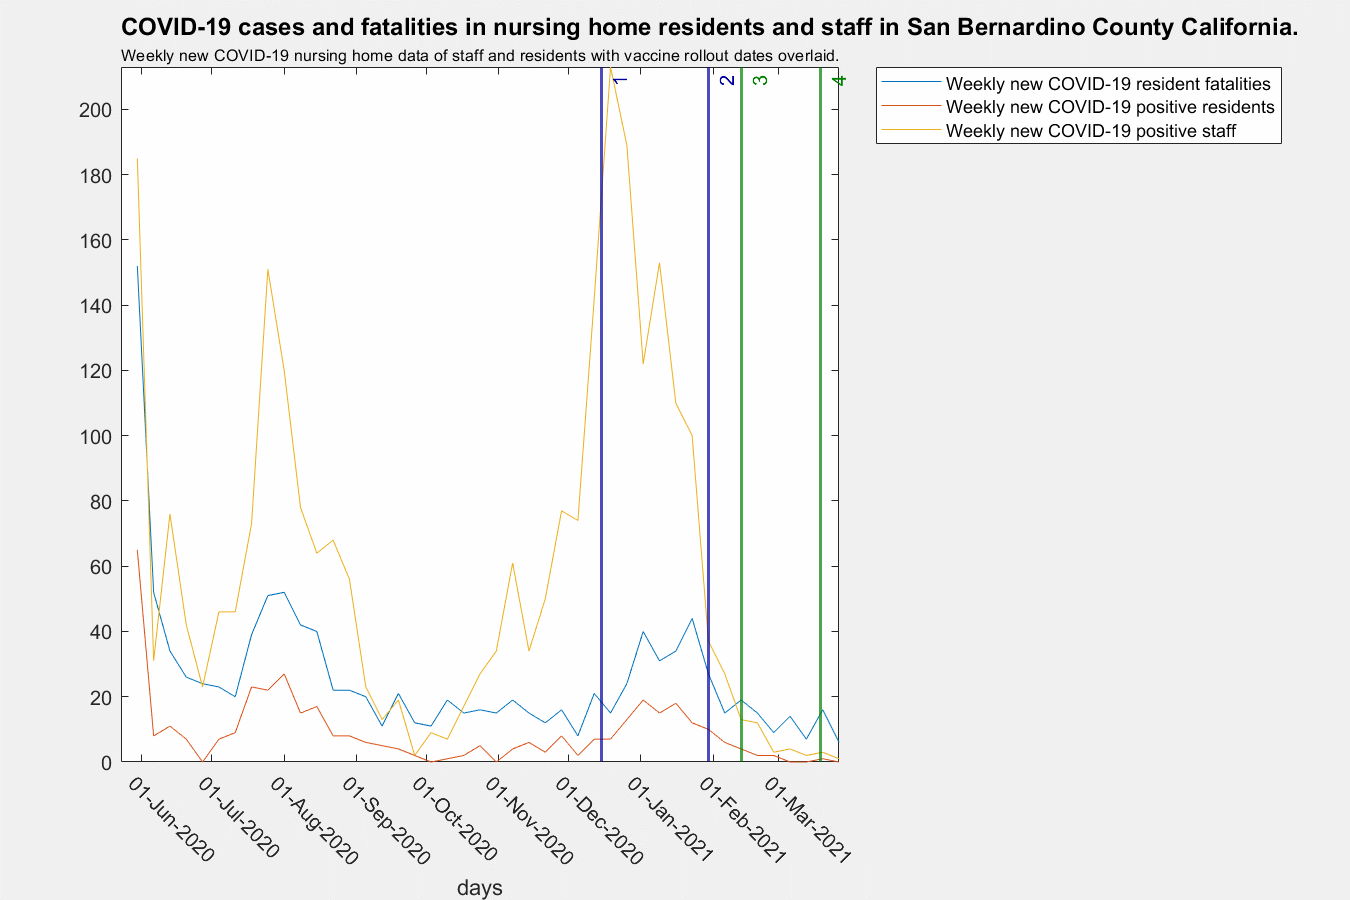
\includegraphics[width=\linewidth]{images/sanbernardino_nursing_home_with_vaccine.png}
	\caption{}
	\label{fig:images/sanbernardino_nursing_home_with_vaccineLabel}
\end{figure}

\begin{figure}[H]
	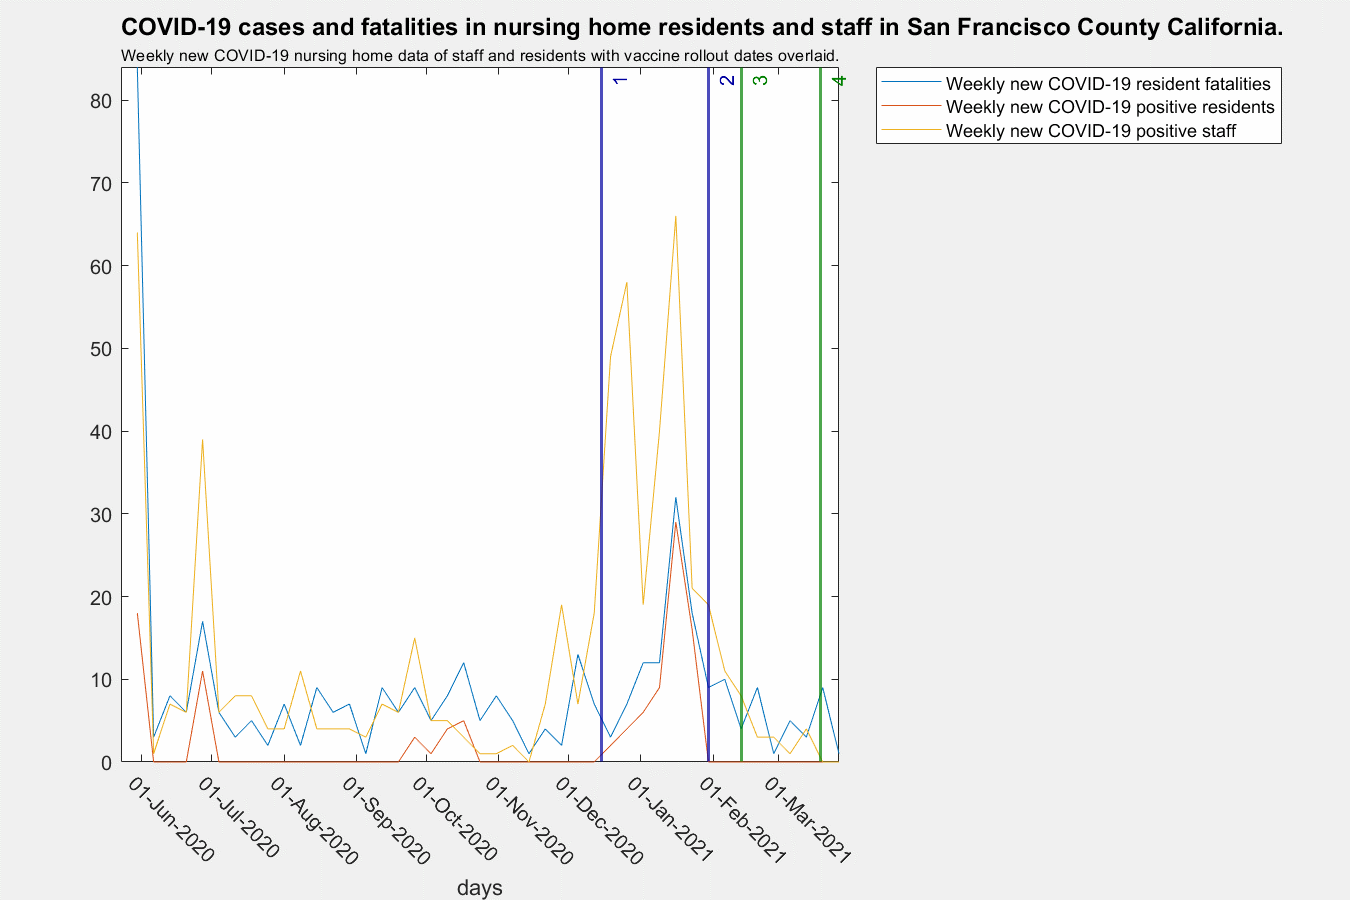
\includegraphics[width=\linewidth]{images/sanfrancisco_nursing_home_with_vaccine.png}
	\caption{}
	\label{fig:images/sanfrancisco_nursing_home_with_vaccineLabel}
\end{figure}

\begin{figure}[H]
	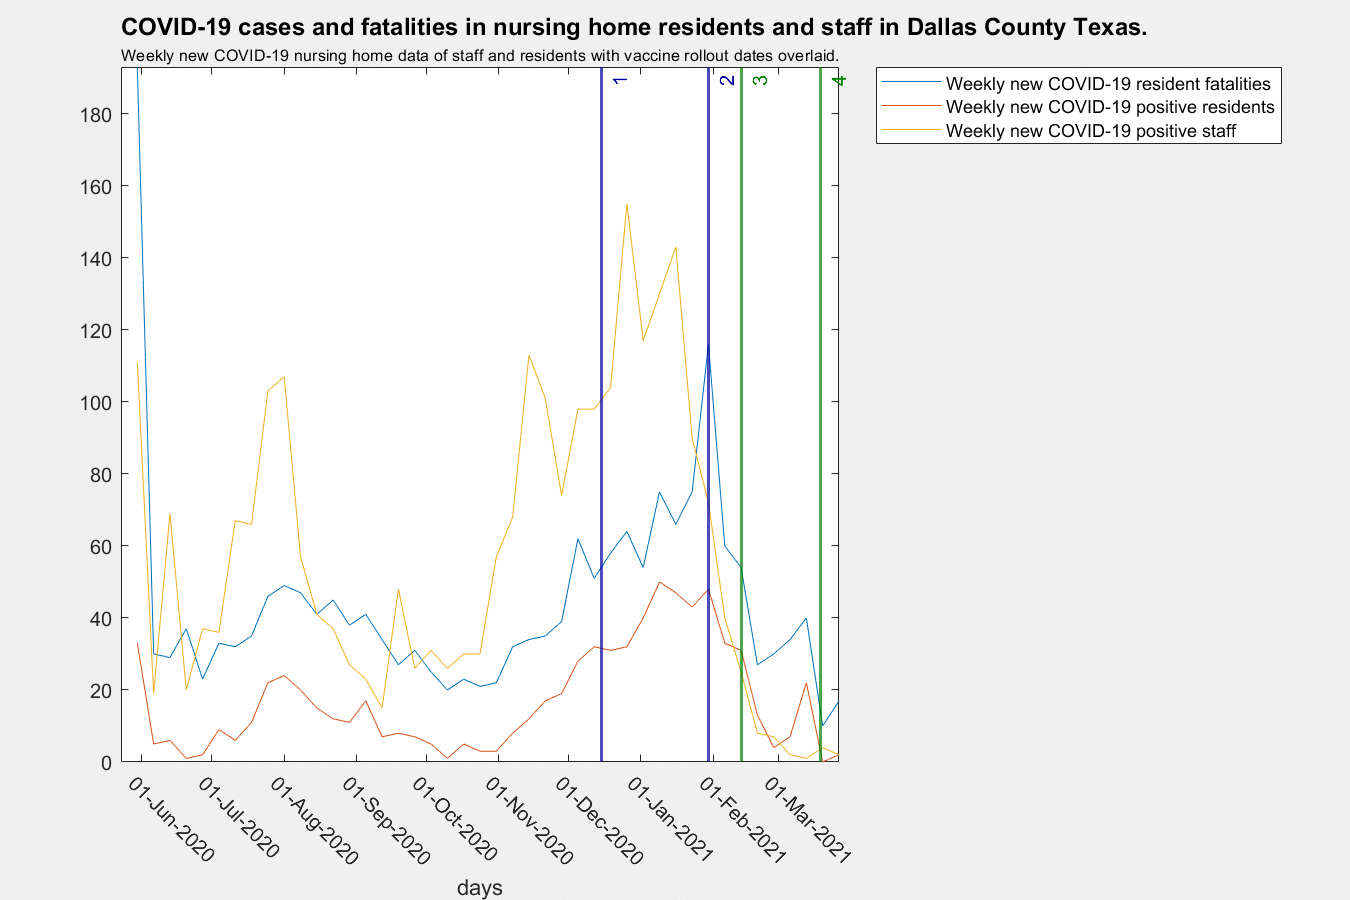
\includegraphics[width=\linewidth]{images/dallas_nursing_home_with_vaccine.png}
	\caption{}
	\label{fig:images/dallas_nursing_home_with_vaccineLabel}
\end{figure}

\begin{figure}[H]
	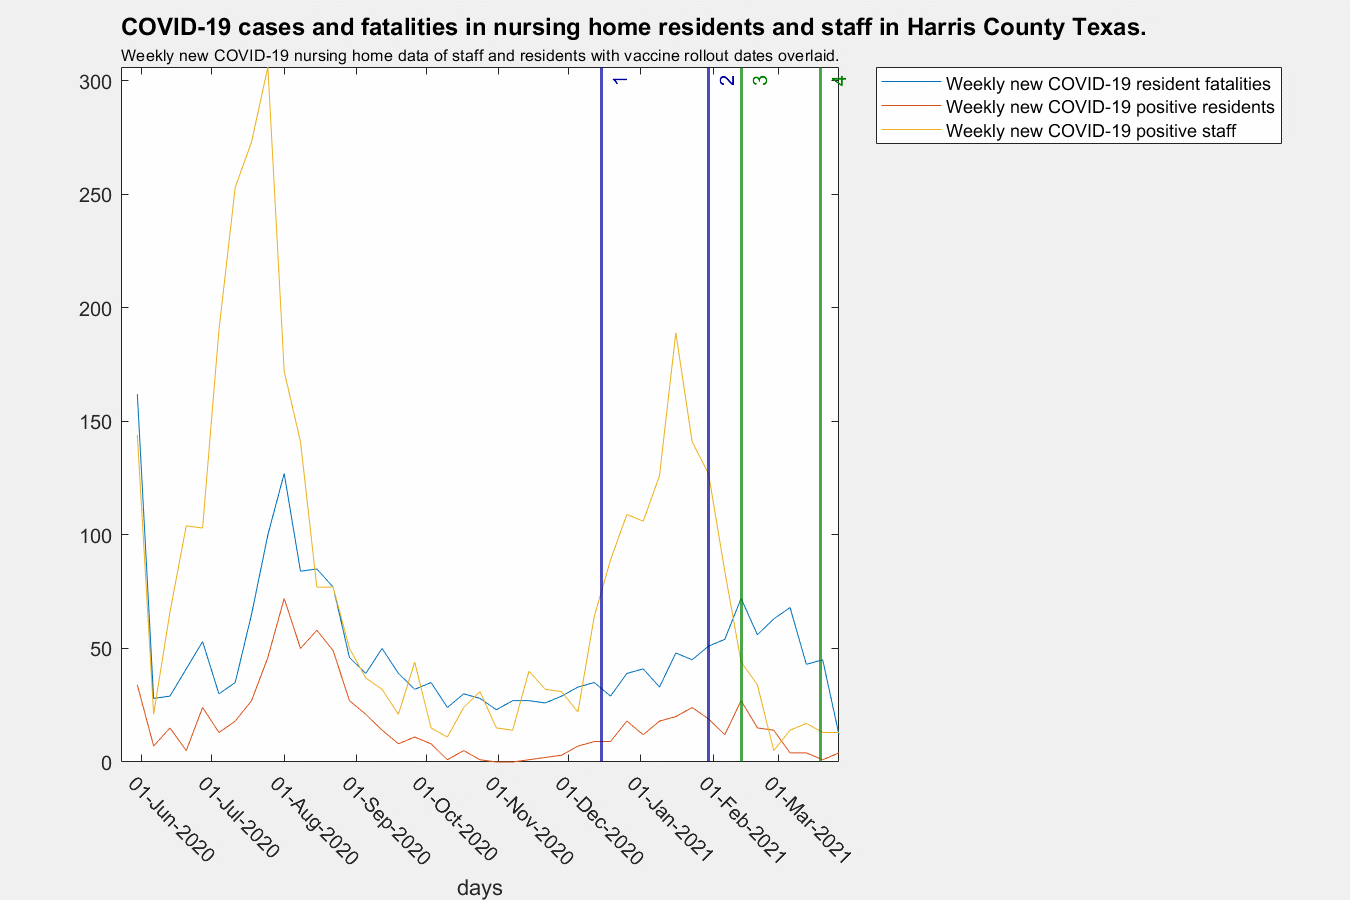
\includegraphics[width=\linewidth]{images/harris_nursing_home_with_vaccine.png}
	\caption{}
	\label{fig:images/harris_nursing_home_with_vaccineLabel}
\end{figure}

\begin{figure}[H]
	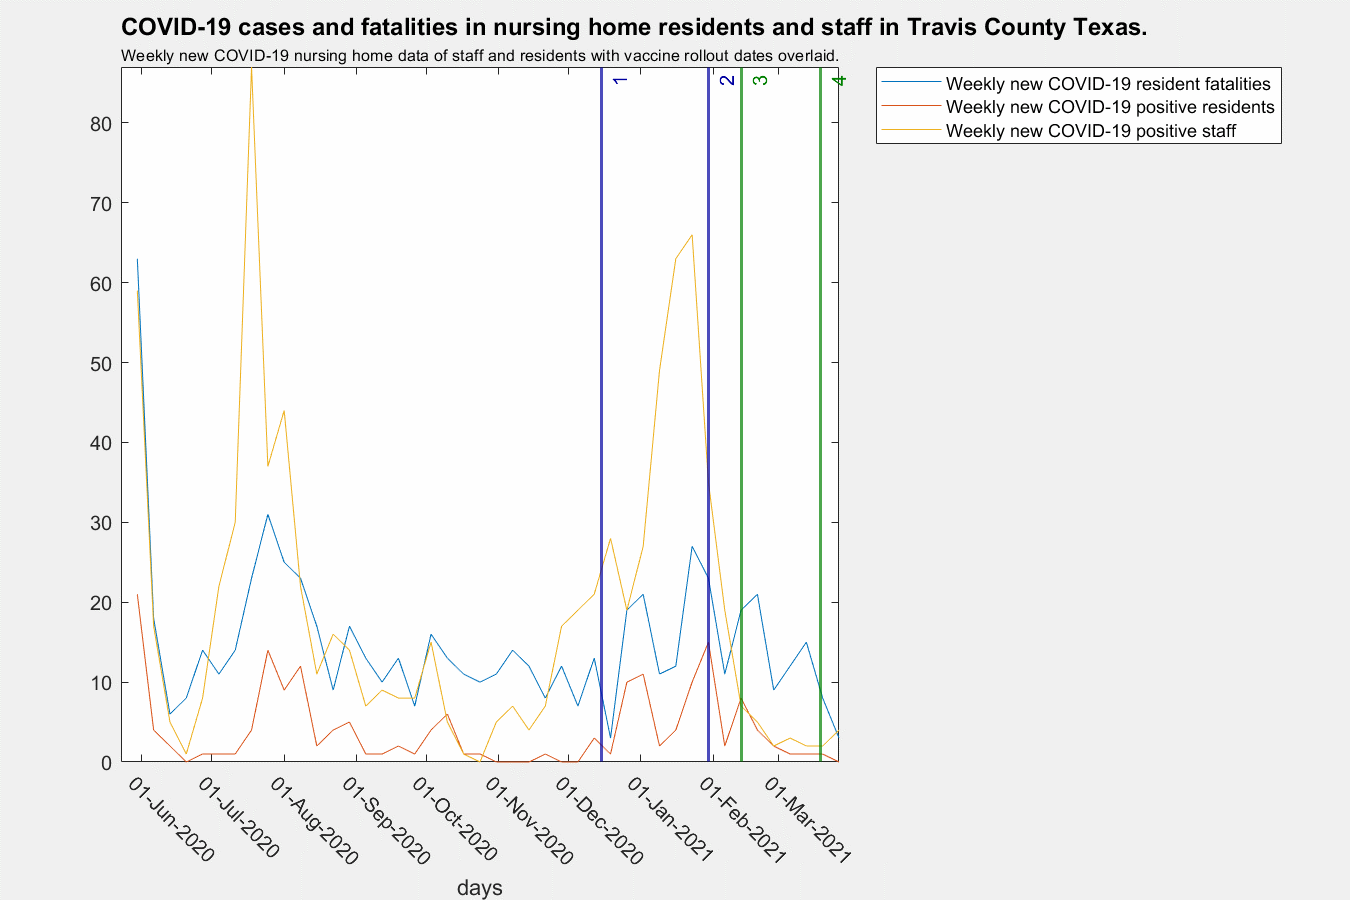
\includegraphics[width=\linewidth]{images/travis_nursing_home_with_vaccine.png}
	\caption{}
	\label{fig:images/travis_nursing_home_with_vaccineLabel}
\end{figure}
\rule{\linewidth}{0.5pt}\\
\subsection{Nursing Home Statistics}


%------------------------------------------------

\section{Discussion}

\subsection{Model Discussion}

\lipsum[7] % Dummy text

\subsection{Event Analysis Discussion}

\lipsum[8] % Dummy text

%----------------------------------------------------------------------------------------
%	REFERENCE LIST
%----------------------------------------------------------------------------------------

\begin{thebibliography}{99} % Bibliography - this is intentionally simple in this template

\bibitem[Figueredo and Wolf, 2009]{Figueredo:2009dg}
Figueredo, A.~J. and Wolf, P. S.~A. (2009).
\newblock Assortative pairing and life history strategy - a cross-cultural
  study.
\newblock {\em Human Nature}, 20:317--330.
 
\end{thebibliography}

%----------------------------------------------------------------------------------------

\end{multicols}

\end{document}